
%% bare_conf.tex
%% V1.4b
%% 2015/08/26
%% by Michael Shell
%% See:
%% http://www.michaelshell.org/
%% for current contact information.
%%
%% This is a skeleton file demonstrating the use of IEEEtran.cls
%% (requires IEEEtran.cls version 1.8b or later) with an IEEE
%% conference paper.
%%
%% Support sites:
%% http://www.michaelshell.org/tex/ieeetran/
%% http://www.ctan.org/pkg/ieeetran
%% and
%% http://www.ieee.org/

%%*************************************************************************
%% Legal Notice:
%% This code is offered as-is without any warranty either expressed or
%% implied; without even the implied warranty of MERCHANTABILITY or
%% FITNESS FOR A PARTICULAR PURPOSE! 
%% User assumes all risk.
%% In no event shall the IEEE or any contributor to this code be liable for
%% any damages or losses, including, but not limited to, incidental,
%% consequential, or any other damages, resulting from the use or misuse
%% of any information contained here.
%%
%% All comments are the opinions of their respective authors and are not
%% necessarily endorsed by the IEEE.
%%
%% This work is distributed under the LaTeX Project Public License (LPPL)
%% ( http://www.latex-project.org/ ) version 1.3, and may be freely used,
%% distributed and modified. A copy of the LPPL, version 1.3, is included
%% in the base LaTeX documentation of all distributions of LaTeX released
%% 2003/12/01 or later.
%% Retain all contribution notices and credits.
%% ** Modified files should be clearly indicated as such, including  **
%% ** renaming them and changing author support contact information. **
%%*************************************************************************


% *** Authors should verify (and, if needed, correct) their LaTeX system  ***
% *** with the testflow diagnostic prior to trusting their LaTeX platform ***
% *** with production work. The IEEE's font choices and paper sizes can   ***
% *** trigger bugs that do not appear when using other class files.       ***                          ***
% The testflow support page is at:
% http://www.michaelshell.org/tex/testflow/



\documentclass[conference]{IEEEtran}
% Some Computer Society conferences also require the compsoc mode option,
% but others use the standard conference format.
%
% If IEEEtran.cls has not been installed into the LaTeX system files,
% manually specify the path to it like:
% \documentclass[conference]{../sty/IEEEtran}





% Some very useful LaTeX packages include:
% (uncomment the ones you want to load)


% *** MISC UTILITY PACKAGES ***
%
%\usepackage{ifpdf}
% Heiko Oberdiek's ifpdf.sty is very useful if you need conditional
% compilation based on whether the output is pdf or dvi.
% usage:
% \ifpdf
%   % pdf code
% \else
%   % dvi code
% \fi
% The latest version of ifpdf.sty can be obtained from:
% http://www.ctan.org/pkg/ifpdf
% Also, note that IEEEtran.cls V1.7 and later provides a builtin
% \ifCLASSINFOpdf conditional that works the same way.
% When switching from latex to pdflatex and vice-versa, the compiler may
% have to be run twice to clear warning/error messages.





\usepackage{url}
% *** CITATION PACKAGES ***
%
\usepackage{cite}
% cite.sty was written by Donald Arseneau
% V1.6 and later of IEEEtran pre-defines the format of the cite.sty package
% \cite{} output to follow that of the IEEE. Loading the cite package will
% result in citation numbers being automatically sorted and properly
% "compressed/ranged". e.g., [1], [9], [2], [7], [5], [6] without using
% cite.sty will become [1], [2], [5]--[7], [9] using cite.sty. cite.sty's
% \cite will automatically add leading space, if needed. Use cite.sty's
% noadjust option (cite.sty V3.8 and later) if you want to turn this off
% such as if a citation ever needs to be enclosed in parenthesis.
% cite.sty is already installed on most LaTeX systems. Be sure and use
% version 5.0 (2009-03-20) and later if using hyperref.sty.
% The latest version can be obtained at:
% http://www.ctan.org/pkg/cite
% The documentation is contained in the cite.sty file itself.






% *** GRAPHICS RELATED PACKAGES ***
%
\ifCLASSINFOpdf
  % \usepackage[pdftex]{graphicx}
  % declare the path(s) where your graphic files are
  % \graphicspath{{../pdf/}{../jpeg/}}
  % and their extensions so you won't have to specify these with
  % every instance of \includegraphics
  % \DeclareGraphicsExtensions{.pdf,.jpeg,.png}
\else
  % or other class option (dvipsone, dvipdf, if not using dvips). graphicx
  % will default to the driver specified in the system graphics.cfg if no
  % driver is specified.
  % \usepackage[dvips]{graphicx}
  % declare the path(s) where your graphic files are
  % \graphicspath{{../eps/}}
  % and their extensions so you won't have to specify these with
  % every instance of \includegraphics
  % \DeclareGraphicsExtensions{.eps}
\fi
% graphicx was written by David Carlisle and Sebastian Rahtz. It is
% required if you want graphics, photos, etc. graphicx.sty is already
% installed on most LaTeX systems. The latest version and documentation
% can be obtained at: 
% http://www.ctan.org/pkg/graphicx
% Another good source of documentation is "Using Imported Graphics in
% LaTeX2e" by Keith Reckdahl which can be found at:
% http://www.ctan.org/pkg/epslatex
%
% latex, and pdflatex in dvi mode, support graphics in encapsulated
% postscript (.eps) format. pdflatex in pdf mode supports graphics
% in .pdf, .jpeg, .png and .mps (metapost) formats. Users should ensure
% that all non-photo figures use a vector format (.eps, .pdf, .mps) and
% not a bitmapped formats (.jpeg, .png). The IEEE frowns on bitmapped formats
% which can result in "jaggedy"/blurry rendering of lines and letters as
% well as large increases in file sizes.
%
% You can find documentation about the pdfTeX application at:
% http://www.tug.org/applications/pdftex





% *** MATH PACKAGES ***
%
%\usepackage{amsmath}
% A popular package from the American Mathematical Society that provides
% many useful and powerful commands for dealing with mathematics.
%
% Note that the amsmath package sets \interdisplaylinepenalty to 10000
% thus preventing page breaks from occurring within multiline equations. Use:
%\interdisplaylinepenalty=2500
% after loading amsmath to restore such page breaks as IEEEtran.cls normally
% does. amsmath.sty is already installed on most LaTeX systems. The latest
% version and documentation can be obtained at:
% http://www.ctan.org/pkg/amsmath





% *** SPECIALIZED LIST PACKAGES ***
%
%\usepackage{algorithmic}
% algorithmic.sty was written by Peter Williams and Rogerio Brito.
% This package provides an algorithmic environment fo describing algorithms.
% You can use the algorithmic environment in-text or within a figure
% environment to provide for a floating algorithm. Do NOT use the algorithm
% floating environment provided by algorithm.sty (by the same authors) or
% algorithm2e.sty (by Christophe Fiorio) as the IEEE does not use dedicated
% algorithm float types and packages that provide these will not provide
% correct IEEE style captions. The latest version and documentation of
% algorithmic.sty can be obtained at:
% http://www.ctan.org/pkg/algorithms
% Also of interest may be the (relatively newer and more customizable)
% algorithmicx.sty package by Szasz Janos:
% http://www.ctan.org/pkg/algorithmicx




% *** ALIGNMENT PACKAGES ***
%
%\usepackage{array}
% Frank Mittelbach's and David Carlisle's array.sty patches and improves
% the standard LaTeX2e array and tabular environments to provide better
% appearance and additional user controls. As the default LaTeX2e table
% generation code is lacking to the point of almost being broken with
% respect to the quality of the end results, all users are strongly
% advised to use an enhanced (at the very least that provided by array.sty)
% set of table tools. array.sty is already installed on most systems. The
% latest version and documentation can be obtained at:
% http://www.ctan.org/pkg/array


% IEEEtran contains the IEEEeqnarray family of commands that can be used to
% generate multiline equations as well as matrices, tables, etc., of high
% quality.



\usepackage{graphicx}
% *** SUBFIGURE PACKAGES ***
%\ifCLASSOPTIONcompsoc
%  \usepackage[caption=false,font=normalsize,labelfont=sf,textfont=sf]{subfig}
%\else
%  \usepackage[caption=false,font=footnotesize]{subfig}
%\fi
% subfig.sty, written by Steven Douglas Cochran, is the modern replacement
% for subfigure.sty, the latter of which is no longer maintained and is
% incompatible with some LaTeX packages including fixltx2e. However,
% subfig.sty requires and automatically loads Axel Sommerfeldt's caption.sty
% which will override IEEEtran.cls' handling of captions and this will result
% in non-IEEE style figure/table captions. To prevent this problem, be sure
% and invoke subfig.sty's "caption=false" package option (available since
% subfig.sty version 1.3, 2005/06/28) as this is will preserve IEEEtran.cls
% handling of captions.
% Note that the Computer Society format requires a larger sans serif font
% than the serif footnote size font used in traditional IEEE formatting
% and thus the need to invoke different subfig.sty package options depending
% on whether compsoc mode has been enabled.
%
% The latest version and documentation of subfig.sty can be obtained at:
% http://www.ctan.org/pkg/subfig



\usepackage{amsmath}
% *** FLOAT PACKAGES ***
%
%\usepackage{fixltx2e}
% fixltx2e, the successor to the earlier fix2col.sty, was written by
% Frank Mittelbach and David Carlisle. This package corrects a few problems
% in the LaTeX2e kernel, the most notable of which is that in current
% LaTeX2e releases, the ordering of single and double column floats is not
% guaranteed to be preserved. Thus, an unpatched LaTeX2e can allow a
% single column figure to be placed prior to an earlier double column
% figure.
% Be aware that LaTeX2e kernels dated 2015 and later have fixltx2e.sty's
% corrections already built into the system in which case a warning will
% be issued if an attempt is made to load fixltx2e.sty as it is no longer
% needed.
% The latest version and documentation can be found at:
% http://www.ctan.org/pkg/fixltx2e


%\usepackage{stfloats}
% stfloats.sty was written by Sigitas Tolusis. This package gives LaTeX2e
% the ability to do double column floats at the bottom of the page as well
% as the top. (e.g., "\begin{figure*}[!b]" is not normally possible in
% LaTeX2e). It also provides a command:
%\fnbelowfloat
% to enable the placement of footnotes below bottom floats (the standard
% LaTeX2e kernel puts them above bottom floats). This is an invasive package
% which rewrites many portions of the LaTeX2e float routines. It may not work
% with other packages that modify the LaTeX2e float routines. The latest
% version and documentation can be obtained at:
% http://www.ctan.org/pkg/stfloats
% Do not use the stfloats baselinefloat ability as the IEEE does not allow
% \baselineskip to stretch. Authors submitting work to the IEEE should note
% that the IEEE rarely uses double column equations and that authors should try
% to avoid such use. Do not be tempted to use the cuted.sty or midfloat.sty
% packages (also by Sigitas Tolusis) as the IEEE does not format its papers in
% such ways.
% Do not attempt to use stfloats with fixltx2e as they are incompatible.
% Instead, use Morten Hogholm'a dblfloatfix which combines the features
% of both fixltx2e and stfloats:
%
% \usepackage{dblfloatfix}
% The latest version can be found at:
% http://www.ctan.org/pkg/dblfloatfix


\usepackage{fixltx2e}

% *** PDF, URL AND HYPERLINK PACKAGES ***
%
%\usepackage{url}
% url.sty was written by Donald Arseneau. It provides better support for
% handling and breaking URLs. url.sty is already installed on most LaTeX
% systems. The latest version and documentation can be obtained at:
% http://www.ctan.org/pkg/url
% Basically, \url{my_url_here}.




% *** Do not adjust lengths that control margins, column widths, etc. ***
% *** Do not use packages that alter fonts (such as pslatex).         ***
% There should be no need to do such things with IEEEtran.cls V1.6 and later.
% (Unless specifically asked to do so by the journal or conference you plan
% to submit to, of course. )


% correct bad hyphenation here
\hyphenation{op-tical net-works semi-conduc-tor}


\begin{document}
%
% paper title
% Titles are generally capitalized except for words such as a, an, and, as,
% at, but, by, for, in, nor, of, on, or, the, to and up, which are usually
% not capitalized unless they are the first or last word of the title.
% Linebreaks \\ can be used within to get better formatting as desired.
% Do not put math or special symbols in the title.
\title{Off you go!}


% author names and affiliations
% use a multiple column layout for up to three different
% affiliations
\author{\IEEEauthorblockN{Sai Chowdary G}
\IEEEauthorblockA{CS 603\\Computational Photography\\
Indian Institute of Technology Gandhinagar\\}
}

% conference papers do not typically use \thanks and this command
% is locked out in conference mode. If really needed, such as for
% the acknowledgment of grants, issue a \IEEEoverridecommandlockouts
% after \documentclass

% for over three affiliations, or if they all won't fit within the width
% of the page, use this alternative format:
% 
%\author{\IEEEauthorblockN{Michael Shell\IEEEauthorrefmark{1},
%Homer Simpson\IEEEauthorrefmark{2},
%James Kirk\IEEEauthorrefmark{3}, 
%Montgomery Scott\IEEEauthorrefmark{3} and
%Eldon Tyrell\IEEEauthorrefmark{4}}
%\IEEEauthorblockA{\IEEEauthorrefmark{1}School of Electrical and Computer Engineering\\
%Georgia Institute of Technology,
%Atlanta, Georgia 30332--0250\\ Email: see http://www.michaelshell.org/contact.html}
%\IEEEauthorblockA{\IEEEauthorrefmark{2}Twentieth Century Fox, Springfield, USA\\
%Email: homer@thesimpsons.com}
%\IEEEauthorblockA{\IEEEauthorrefmark{3}Starfleet Academy, San Francisco, California 96678-2391\\
%Telephone: (800) 555--1212, Fax: (888) 555--1212}
%\IEEEauthorblockA{\IEEEauthorrefmark{4}Tyrell Inc., 123 Replicant Street, Los Angeles, California 90210--4321}}




% use for special paper notices
%\IEEEspecialpapernotice{(Invited Paper)}




% make the title area
\maketitle

% As a general rule, do not put math, special symbols or citations
% in the abstract
\begin{abstract}
The popularity of Digital photography has been rising rapidly in the recent times. A large number of photographs being taken everyday, everything from special events to normal day to day activities are being captured. The proliferation of smart phones with quality inbuilt cameras has especially helped this observed trend. The most commonly captured scenes are those of monuments, natural scenes, parties or indoor activities etc by tourists, guests etc. But in most of these images due to the nature of the scene being captured the object of interest often gets occluded, for example the monument being captured might get occluded by other tourists who are moving about. In such cases one can capture multiple images of the scene such that the information lost in one image of the object of interest is available in the other image. In this project an attempt is made to remove such occluding objects and inpainting the image with the information of interest from the other image of the same scene using the principles of Homography, Laplacian Blending, Seam Carving etc.    
\end{abstract}

% no keywords




% For peer review papers, you can put extra information on the cover
% page as needed:
% \ifCLASSOPTIONpeerreview
% \begin{center} \bfseries EDICS Category: 3-BBND \end{center}
% \fi
%
% For peerreview papers, this IEEEtran command inserts a page break and
% creates the second title. It will be ignored for other modes.
\IEEEpeerreviewmaketitle



\section{Introduction}
% no \IEEEPARstart
	Of late due to the technological advancements it has become possible to have good quality inbuilt digital cameras because of this there has been a large increase in the number of digital photographs being captured. One of the common problem that vexes people is that of occlusion i.e the object of interest in the scene is often occluded (covered) by other objects in the scene or other people etc. If it is some monument or a famous building, chances are that you will not be able to capture it completely as almost surely there will be other tourists around you who are trying to capture the building from different views and it would be a herculean task to get all of them out of your frame of view so how much ever we try these people will end up occluding some part of the building or the other. Or in some other cases we might want to be the only person in the photo like at a party scene etc but here too some other people might come invariably be captured into the image along with you (though this can not exactly be called as occlusion, we would still prefer to not have such objects in the image). In some other case, from an old photograph of some house etc we might want to remove some objects or people occluding it in the image so that we have the complete place in the captured. 
	From the above scenarios it is clear that there are a large number of photographs from which we would like to remove the occluding objects and try to fill up that patch by what should actually have been there had the occluding object not been present while capturing the image. One simple solution would to crop the object from the scene if possible, or even better remove the object using seam carving[], while this solution does succeed in removing the unwanted objects it does not give the original information of the object of interest that we want, it just throws away the unwanted stuff, moreover in some cases this can distort the object of interest as well (this can happen when the amount of occlusion is high). To address this issue we need to some how get the actual information of the occluded part, this can indeed be obtained from another image of the same scene but taken from a different view(it is also possible to get the lost information from an image taken from the same view but a after some time as the object if it is a person might move to a different point and will not be occluding the previous patch now). Then we must replace the occluding object with this information by inpainting.
	We use Homography to geometrically align the images, then we find the patch to be replace the occluding object using the computed Homography and then combine this patch with the original image using laplacian blending. Also in case the images are capture by different cameras or lighting conditions this would make the final result less appealing so to account for this we come up with a multiplication factor to adjust the luminance values. 
\section{Related Works}	  
	This implementation follows the rough outline of the technique suggested by [\cite{whyte2009get}] though many changes have been made to it. Previous works of image Inpainting vary a lot in their efficiency depending on various factors like the surroundings of the region to be filled, and the size of the region to be filled. For a few algorithms[\cite{bertalmio2003simultaneous},\cite{efros1999texture}] if the size of the region is small enough then using the surrounding information we can fill the region but this will fail in the case of larger regions that need to be filled. To account for this new algorithms[\cite{bertalmio2003simultaneous},\cite{criminisi2003object},\cite{sun2005image}] have been proposed which take into consideration the salient structures and textures across the region. But still they do not perform to our satisfaction as in all these cases we only try to predict the region to be filled from the one occluded image that we possess. A few algorithms[\cite{agarwala2004interactive},\cite{rasmussen2005spatiotemporal},\cite{wilczkowiak2005hole}] use the images of the same scene but under the constraint that the images be captured by the same camera.
	Using this technique we can fill regions of almost any size and also the images need not be of the same camera as long the object of interest is almost planar(minor depth variations will not be an issue). 
% You must have at least 2 lines in the paragraph with the drop letter
% (should never be an issue)
\section{Proposed Approach}
	Two images are sufficient to implement the proposed approach, if we have more than two images even then the same approach is followed but we have to repeat it multiple times by taking one fixed reference image and changing the other image. So in the following subsections we will discuss the approach as though we have only two images.
\subsection{Geometric Alignment: Homography}
	As we have discussed, if we have images of the scene from different views we can then remove the occluding object and try to fill up the patch with the correct pixels from the other image, so we need to find a geometrical transformation to relate pixels in the two images. A homography transform []is a 3 $\times$ 3 full rank matrix that maps points from one plane to another. It is interesting to note that while if the scene of interest is planar as is the case with many buildings then we can easily map the two views with a homography, also more importantly even if the scene is not planar but if the camera center has not been changed even then both the scenes are related by a homography as proved in[\cite{hartley2003multiple}].
%	\left[ \begin{array}{c} x_1 \\ y_1 \\ z1 \end{array} \right] = \begin{bmatrix} h_11 & h_12 & h_13\\ h_21 & h_22 & h_23 \\h_31 & h_32 & h_33\end{bmatrix} \times \left[ \begin{array}{c} x_2 \\ y_2\\ 1 \end{array} \right]
\[
  \begin{pmatrix} x_1 \\ y_1\\z_1 \end{pmatrix} = 
  \begin{pmatrix} h_11 & h_12 & h_13\\ h_21 & h_22 & h_23\\ h_31 & h_32 & h_33 \end{pmatrix} 
  \begin{pmatrix} x_2 \\ y_2\\1 \end{pmatrix}
\]

\[\begin{pmatrix} x_1 & y_1 & z_1 \end{pmatrix} -pixel\quad coordinates\quad in\quad 1st\quad image\] 
\[\begin{pmatrix} x_2 & y_2 & 1 \end{pmatrix} -pixel\quad coordinates\quad in\quad 2nd\quad image\] 
	Now if the camera center does not exactly remain the same but moves slightly, then as long as this movement is reasonably small compared to depths of objects in the scene even then we make the assumption that there will still be a reasonably good homography mapping existing between the scenes even but we will have to accomodate a small translation to account for the motion of the camera as well. This kind of a scenario occurs mostly in the ubiquitous case of hand-held mobile cameras. However if the motion of the camera is too much then there will be unpleasant warping induced in the scene so care must be take that the camera center is not shifted by much. If the scene is planar we can go even further in that we can take images of the same scene by some other camera (of course from different view points) as well, this means that we can use the vast amount of images present in the internet as well so this would be a very convenient case for us. Once we have a set of images that satisfy our above criteria then we find the point correspondences between them and then estimate the homography matrix $H$ [\cite{hartley2003multiple}]. Once $H$ is estimated between two of the given images we then create a mask such that it will remove the occluding object from the first image (i.e masking it with black), and then using $H$ we align the pixels in the other image. Now mask the first image and blend it with second image accordingly.     
\subsection{Blending: Laplacian}
	We use Laplacian Blending to combine both the aligned images and a manually defined mask that masks the occluding object, for this first the gaussian pyramids are created for both the images and from these we obtain their laplacian pyramids as the difference of gaussians at each level, the gaussian pyramid of the mask is computed and from these the laplacian pyramid for the blended image is calculated for each level $ i$ as :\\
	L\textsubscript{result,i}=G\textsubscript{mask,i} $\times$L \textsubscript{image1,i}+1-G\textsubscript{mask,i} $\times$L \textsubscript{image2,i}
\\	L \textsubscript{result,i}: Laplacian pyramid of the result image at level $i$.
\\	L \textsubscript{image1,i}: Laplacian pyramid of the image 1 at level $i$.
\\ 	L \textsubscript{image2,i}: Laplacian pyramid of the image 2 at level $i$.
\subsection{Luminance factor}
	If the two images are taken by different cameras or at different times or in different lighting conditions then the same corresponding regions in both the images will have different intensity values so just transferring the pixels from one image to the other will give us a result that is not visually appealing even after laplacian blending. To counter this we introduce a luminance factor, both the images are converted from RGB colorspace to CIELab colorspace then the average luminance is calculated in both the images and the ratio of these is taken which is the Luminance factor. We multiply L channel of the appropriate image with this factor and then perform laplacian blending. 

\subsection{Seam Carving}
	It often happens that the second image might not be able to completely fill in the patch caused by the object that has been removed this leaves some black patches in the result one way to get rid of these is to add seams accordingly, this however was found to be a very unappealing, due to the addition of seams the transferred pixels get shifted in the vertical or horizontal directions and this causes discontinuities in the previously perfectly aligned edges and other features across the patch boundary. So we instead decrease the energy of the unfilled portion of the patch and remove it using seam carving[\cite{avidan2007seam}]. The minimum energy seams (which will include the unfilled portion of the patch) are removed and
we get our final result.
\section{Results}
\begin{figure}
  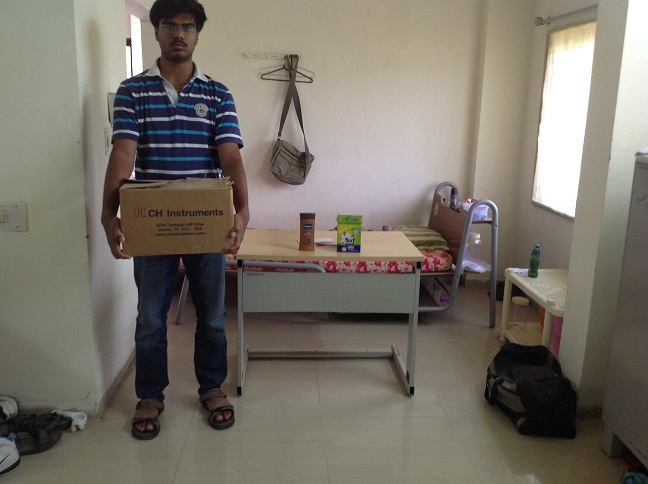
\includegraphics[width=\linewidth]{img1.jpg}
  \caption{Image 1.}
  \label{fig:i1}
\end{figure}
\begin{figure}
  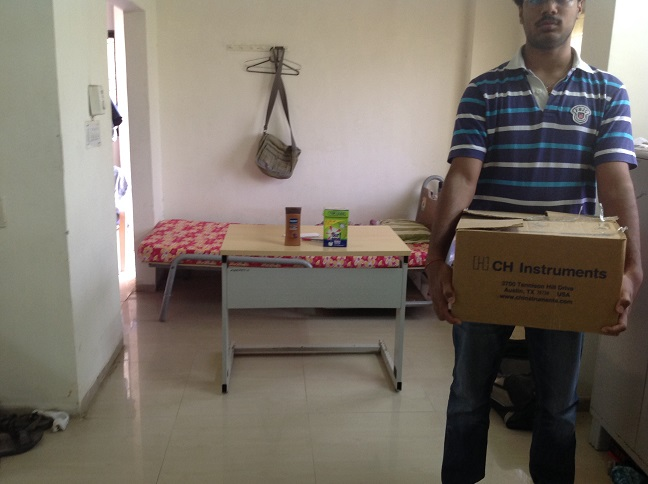
\includegraphics[width=\linewidth]{img2.jpg}
  \caption{Image 2.}
  \label{fig:i2}
\end{figure}
	Consider the dataset of two images Fig.1 and Fig.2, Our task is to get a complete image of the room, the person is currently occluding the room in both the images, but as the person was moving and his position has changed the information occluded in one image is available in the other image for both the images as the person was moving and his position has changed. Also it is known that the camera was not moved much while in between capturing the two images so we can find a homography transformation $H$ between the two images. the $H$ matrix is found and the second image is aligned with the first image as shown in Fig.3.
\begin{figure}
  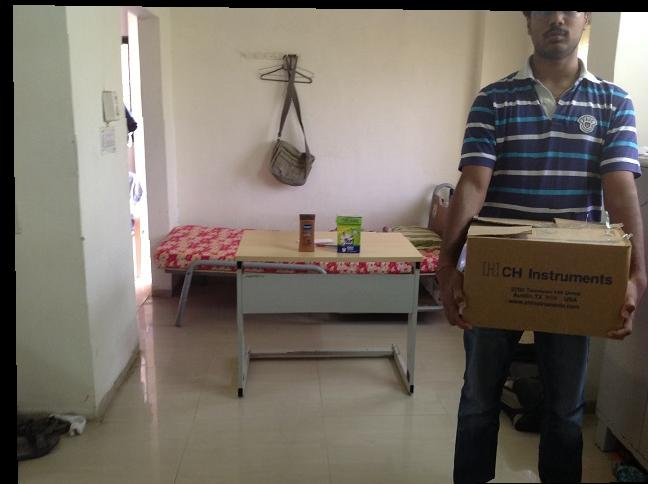
\includegraphics[width=\linewidth]{h.jpg}
  \caption{Geometrically aligned image 2.}
  \label{fig:i3}
\end{figure}
	Also as the images were captured by the same camera and under similar lighting conditions we need not bother about the luminance factor in this case, in fact it was computed and was found to be almost unity and its inclusion did not change the visual perceptibility so it was not considered for this dataset. Initially the pixels are transfered just using the $H$ matrix to obtain the result as shown in Fig.5. We remove the entire block of the image which has the person in it, here we have manually decided what the patch has to be as shown in Fig.4. As we can see, the patch is replaced by the part of the wall that would actually have been there if not for the occlusion. So we are able to perform the inpainting using homography. But if we observe Fig.5 closely the result is not visually very appealing as the boundary of the patch which was removed are clearly visible and i.e is no smooth transition at the boundary of the patch. 
\begin{figure}
  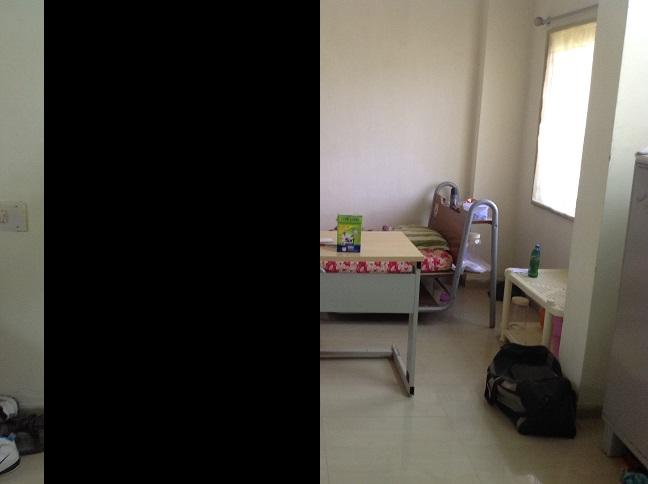
\includegraphics[width=\linewidth]{patch.jpg}
  \caption{Image 1 with the patch to be filled.}
  \label{fig:i4}
\end{figure}
\begin{figure}
  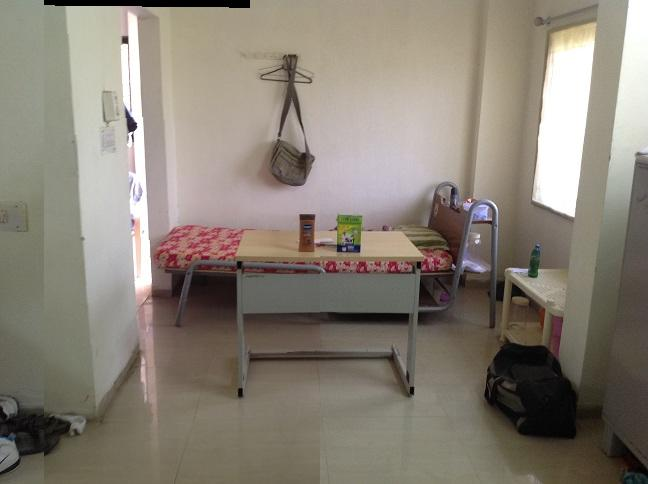
\includegraphics[width=\linewidth]{wb.jpg}
  \caption{Result of directly transferring the pixels without Laplacian Blending.}
  \label{fig:i5}
\end{figure}
	So instead of directly transferring the pixels we perform laplacian blending between the geometrically aligned Image 2 and Image 1 with the appropriate mask to remove the patch. We can see the result of this operation in Fig.6. We see that though it is visually much better than Fig.5, Fig.6 still has some parts of the patch unfilled as the image 2 does not have that information. So we perform Seam carving after assigning very low and negative energy to pixels corresponding to unfilled parts of the patch to remove it. Fig.7 is the final result obtained. 

\begin{figure}
  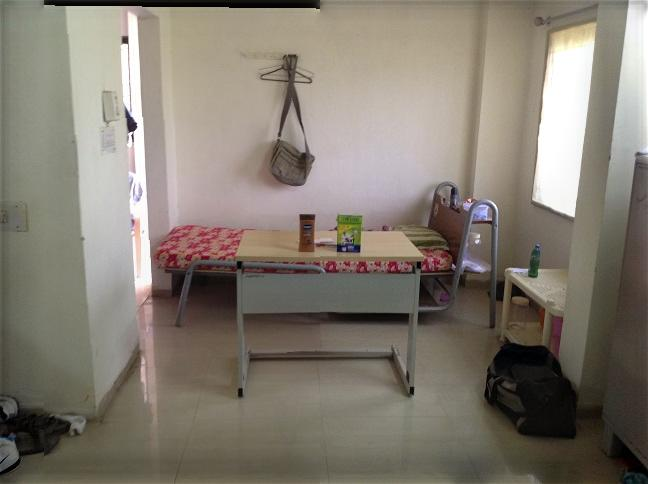
\includegraphics[width=\linewidth]{ab.jpg}
  \caption{Result after Laplacian Blending.}
  \label{fig:i6}
\end{figure}
\begin{figure}
  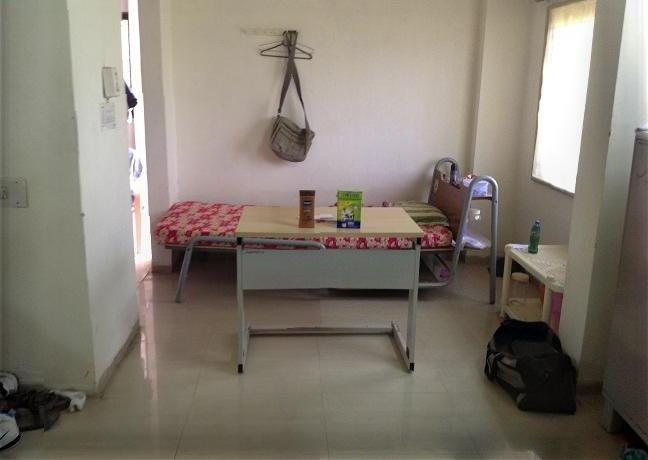
\includegraphics[width=\linewidth]{result.jpg}
  \caption{Final Result after Seam Carving.}
  \label{fig:i7}
\end{figure}


% An example of a floating figure using the graphicx package.
% Note that \label must occur AFTER (or within) \caption.
% For figures, \caption should occur after the \includegraphics.
% Note that IEEEtran v1.7 and later has special internal code that
% is designed to preserve the operation of \label within \caption
% even when the captionsoff option is in effect. However, because
% of issues like this, it may be the safest practice to put all your
% \label just after \caption rather than within \caption{}.
%
% Reminder: the "draftcls" or "draftclsnofoot", not "draft", class
% option should be used if it is desired that the figures are to be
% displayed while in draft mode.
%
%\begin{figure}[!t]
%\centering
%\includegraphics[width=2.5in]{myfigure}
% where an .eps filename suffix will be assumed under latex, 
% and a .pdf suffix will be assumed for pdflatex; or what has been declared
% via \DeclareGraphicsExtensions.
%\caption{Simulation results for the network.}
%\label{fig_sim}
%\end{figure}

% Note that the IEEE typically puts floats only at the top, even when this
% results in a large percentage of a column being occupied by floats.


% An example of a double column floating figure using two subfigures.
% (The subfig.sty package must be loaded for this to work.)
% The subfigure \label commands are set within each subfloat command,
% and the \label for the overall figure must come after \caption.
% \hfil is used as a separator to get equal spacing.
% Watch out that the combined width of all the subfigures on a 
% line do not exceed the text width or a line break will occur.
%
%\begin{figure*}[!t]
%\centering
%\subfloat[Case I]{\includegraphics[width=2.5in]{box}%
%\label{fig_first_case}}
%\hfil
%\subfloat[Case II]{\includegraphics[width=2.5in]{box}%
%\label{fig_second_case}}
%\caption{Simulation results for the network.}
%\label{fig_sim}
%\end{figure*}
%
% Note that often IEEE papers with subfigures do not employ subfigure
% captions (using the optional argument to \subfloat[]), but instead will
% reference/describe all of them (a), (b), etc., within the main caption.
% Be aware that for subfig.sty to generate the (a), (b), etc., subfigure
% labels, the optional argument to \subfloat must be present. If a
% subcaption is not desired, just leave its contents blank,
% e.g., \subfloat[].


% An example of a floating table. Note that, for IEEE style tables, the
% \caption command should come BEFORE the table and, given that table
% captions serve much like titles, are usually capitalized except for words
% such as a, an, and, as, at, but, by, for, in, nor, of, on, or, the, to
% and up, which are usually not capitalized unless they are the first or
% last word of the caption. Table text will default to \footnotesize as
% the IEEE normally uses this smaller font for tables.
% The \label must come after \caption as always.
%
%\begin{table}[!t]
%% increase table row spacing, adjust to taste
%\renewcommand{\arraystretch}{1.3}
% if using array.sty, it might be a good idea to tweak the value of
% \extrarowheight as needed to properly center the text within the cells
%\caption{An Example of a Table}
%\label{table_example}
%\centering
%% Some packages, such as MDW tools, offer better commands for making tables
%% than the plain LaTeX2e tabular which is used here.
%\begin{tabular}{|c||c|}
%\hline
%One & Two\\
%\hline
%Three & Four\\
%\hline
%\end{tabular}
%\end{table}


% Note that the IEEE does not put floats in the very first column
% - or typically anywhere on the first page for that matter. Also,
% in-text middle ("here") positioning is typically not used, but it
% is allowed and encouraged for Computer Society conferences (but
% not Computer Society journals). Most IEEE journals/conferences use
% top floats exclusively. 
% Note that, LaTeX2e, unlike IEEE journals/conferences, places
% footnotes above bottom floats. This can be corrected via the
% \fnbelowfloat command of the stfloats package.




\section{Conclusion}
	Thus using this technique we can inpaint regions of any size as long as we have another image which can supply the information regarding the occluded part. We are able to obtain a visually pleasing inpainted image from the two given images after removing the occluding object. Thus  using homography 
proves to be a nice technique for inpainting, other correspondences techniques like NRDC[] were also tried but the results were not satisfactory. One potential improvement could be making the generation of the mask automatic, we can probably achieve this by finding seams along which the intensity variation is very less between the two images as is done in Photomontage[\cite{agarwala2004interactive}]. 



% conference papers do not normally have an appendix


% use section* for acknowledgment


% trigger a \newpage just before the given reference
% number - used to balance the columns on the last page
% adjust value as needed - may need to be readjusted if
% the document is modified later
%\IEEEtriggeratref{8}
% The "triggered" command can be changed if desired:
%\IEEEtriggercmd{\enlargethispage{-5in}}

% references section

% can use a bibliography generated by BibTeX as a .bbl file
% BibTeX documentation can be easily obtained at:
% http://mirror.ctan.org/biblio/bibtex/contrib/doc/
% The IEEEtran BibTeX style support page is at:
% http://www.michaelshell.org/tex/ieeetran/bibtex/
%\bibliographystyle{IEEEtran}
% argument is your BibTeX string definitions and bibliography database(s)
%\bibliography{IEEEabrv,../bib/paper}
%
% <OR> manually copy in the resultant .bbl file
% set second argument of \begin to the number of references
% (used to reserve space for the reference number labels box)
\bibliographystyle{IEEEtran}
\bibliography{refs}
%\begin{thebibliography}{1}

%\bibitem{IEEEhowto:kopka}
%H.~Kopka and P.~W. Daly, \emph{A Guide to \LaTeX}, 3rd~ed.\hskip 1em plus
%  0.5em minus 0.4em\relax Harlow, England: Addison-Wesley, 1999.
%\bibitem{} 
%URL
%\\\texttt{http://www.di.ens.fr/willow/research/inpainting/}
%\bibitem{} 
%URL
%\\\texttt{http://www.di.ens.fr/willow/research/inpainting/}
%URL
%\\\texttt{http://www.robots.ox.ac.uk/~vgg/research/oxbuildings/}
%\bibit
%\end{thebibliography}
%
%[4] A. Agarwala, M. Dontcheva, M. Agrawala, S. Drucker, A. Colburn, B. Curless, D. Salesin, and
%M. Cohen. Interactive digital photomontage. ACM Trans. Graphics (Proc. SIGGRAPH 2004),
%23(3):294–302, 2004.
%[5] H. Amirshahi, S. Kondo, and T. Aoki. Photo completion using images from internet photo sharing
%sites. In Proc. MIRU, 2007.
%[6] H. Amirshahi, S. Kondo, K. Ito, and T. Aoki. An image completion algorithm using occlusionfree
%images from internet photo sharing sites. IEICE Trans. Fundamentals of Electronics, Communications
%and Computer Sciences, E91-A(10):2918–2927, 2008.
%



% that's all folks
\end{document}


